\documentclass[journal,hidelinks]{IEEEtran}
\usepackage[utf8]{inputenc}
\usepackage[
  pdftitle={A Practical Analysis of the Convergence of Back Propagation},
  pdfauthor={Andrei Purcarus and Sean Stappas},
  pdfsubject={ECSE-526 -- Artificial Intelligence}
]{hyperref}
\usepackage{graphicx}
\usepackage[all]{hypcap}
\usepackage[noabbrev,capitalize,nameinlink]{cleveref}
\usepackage{indentfirst}
\usepackage[per-mode=symbol]{siunitx}
\usepackage{todonotes}

\title{A Practical Analysis of the Convergence \\ of Back Propagation}
\author{Andrei~Purcarus,~\IEEEmembership{McGill~University} and Sean~Stappas,~\IEEEmembership{McGill~University}}

\begin{document}
\sloppy

\maketitle

\begin{abstract}

A vectorized version of the back propagation algorithm for fully connected artificial neural networks was implemented in order to provide a practical analysis of its convergence. Several improvements, such as input normalization, the use of the hyperbolic tangent as an activation function, and the use of a larger batch size in stochastic gradient descent, were found to be effective in reducing training time. Other improvements, such as reducing the learning rate for higher layers in the network, were found to be ineffective for shallow networks. Several improvements were also suggested to allow for the study of the convergence of back propagation for deeper networks.

\end{abstract}

\section{Introduction}

\IEEEPARstart{T}{his} report provides a practical analysis of the convergence of the back propagation algorithm for a fully connected neural network. To provide this analysis, we first implemented a vectorized version of the back propagation algorithm for a fully connected network of arbitrary size. Then, we applied a series of ``tricks of the trade'' to try to speed up the convergence of the algorithm. Finally, we compared our best results to those of a deep convolutional network and of a random baseline.

\section{Implementation of a Fully Connected Network}

We started by implementing a fully connected neural network in Python. Our starting point was the traditional back propagation algorithm given in AI textbooks \cite{russell_ai_2009}. However, in order to obtain good performance out of the network and avoid the interpretation overhead of Python, we decided to vectorize the algorithm and take advantage of the efficient matrix multiplication implementation provided by NumPy.

Assuming we have a network with $k$ layers, we label the bias weight vectors as $b_j$ and the weight matrices as $W_j$, for $j = 1, \cdots, k-1$. In addition, we label our activation function as $f$, the input vector as $x$, and the expected output vector as $y$. The algorithm then proceeds as follows:
\begin{enumerate}
  \item Forward propagate the input $x$ through the network, saving the intermediate values $in_j$ and $out_j$ for every layer.
  \item Compute the matrix $\Delta$ using
    \begin{equation}
    \Delta_{k-1} = f'(in_k) \cdot (y - out_k)
    \end{equation}
  \item Back propagate the matrix $\Delta$ through the network using
    \begin{equation}
    \Delta_j = f'(in_{j+1}) \cdot W_{j+1}^T \Delta_{j+1}, \  j = 1, \cdots, k-2
    \end{equation}
  \item Compute the gradient of the mean squared error function with regularization using
    \begin{equation}
    \frac{\partial E}{\partial b_j} = -\Delta_j + \lambda b_j, \  j = 1, \cdots, k-1
    \end{equation}
    \begin{equation}
    \frac{\partial E}{\partial W_j} = -\Delta_j out_j^T + \lambda W_j, \  j = 1, \cdots, k-1
    \end{equation}
where $\lambda$ is a regularization parameter that penalizes large weights.
\end{enumerate}
The gradient can then be used to perform gradient descent and train the network.

\section{MNIST Data Set}

We next had to select a data set to perform our experiments on. We chose the widely used MNIST data set, which consists of a set of $60,000$ hand written digits that serve as training examples and $10,000$ hand written digits that serve as test examples. A sample of this data set is shown in \Cref{fig:mnist}. This set provided us with a large amount of data to test our neural network with.

\begin{figure}[!htb]
  \centering
  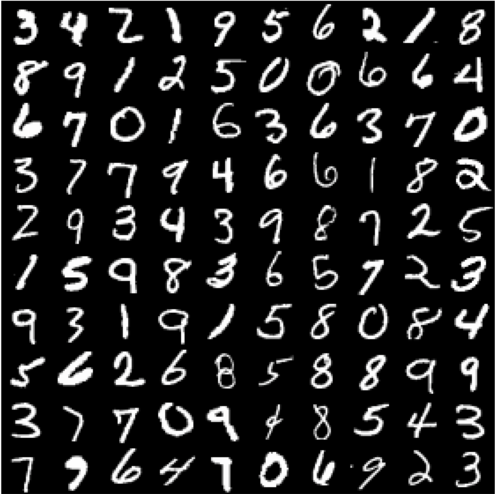
\includegraphics[width=0.8\columnwidth]{figures/mnist.png}
  \caption{Sample digits from the MNIST data set \cite{steeves_2015}.}
  \label{fig:mnist}
\end{figure}

\section{Convergence Improvements}

We next moved to analyzing the convergence of back propagation when using stochastic gradient descent. The majority of the improvements in this section are drawn from LeCun's 1998 paper \textit{Efficient BackProp} \cite{lecun_efficient_1998}, which provided an analysis of several ``tricks of the trade'' and how they improve convergence. Unless otherwise specified, we used a single hidden layer containing $100$ nodes, the hyperbolic tangent activation function, a learning rate of $0.01$, a batch size of $100$, and no momentum.

\subsection{Input Normalization}

To speed up convergence, every node in every layer should have an input with an average close to zero. This ensures that the weight updates during learning are not biased in any particular direction. In addition, the input to each node should have the same standard deviation in order to equalize the learning speed across nodes. To achieve this, the input normalization, activation function, and weight initialization must be carefully coordinated \cite{lecun_efficient_1998}.

First, we normalize the input training data through shifting and scaling. To ensure that the mean of the input data is zero, we subtract the mean of the input vectors from each input vector, using \Cref{eq:normalization_mean}.

\begin{equation} \label{eq:normalization_mean}
x_i \leftarrow x_i - \bar{x}
\end{equation}

Once the mean is subtracted, we divide each input vector by the standard deviation $\sigma_x$ of the input vectors using \Cref{eq:normalization_variance}. This ensures a variance of $1$ over the input data.

\begin{equation} \label{eq:normalization_variance}
x_i \leftarrow \frac{x_i}{\sigma_{x}}
\end{equation}

The parameters $\bar{x}$ and $\sigma_x$ must be stored and later applied to the test input data once training is complete.

\subsection{Sigmoid}

The choice of activation function is also important to ensure optimal convergence. We compare two sigmoid functions: the logistic sigmoid function and the hyperbolic tangent sigmoid function. The logistic sigmoid function is given by \Cref{eq:sigmoid_logistic}.

\begin{equation} \label{eq:sigmoid_logistic}
f_{logistic}(x) = \frac{1}{1 + e^{-x}}
\end{equation}

The hyperbolic tangent sigmoid function is given by \Cref{eq:sigmoid_tanh}. This function is recommended by LeCun for several reasons \cite{lecun_efficient_1998}. First, it is symmetric around the origin and therefore does not induce any bias. The output variance will also be close to $1$ if the input variance is $1$. Next, it has the property that $f(\pm1) = \pm1$ and that $\pm 1$ are not asymptotes. In fact, these are points where the second derivative has a maximum. Therefore, the input as well as the target values of the sigmoid can be safely initialized in the full range from $-1$ to $+1$. This is in contrast with the logistic sigmoid, where target values of $\pm1$ cannot be used because they are asymptotes.

\begin{equation} \label{eq:sigmoid_tanh}
f_{tanh}(x) = 1.7159 \tanh \left( \frac{2}{3} x \right)
\end{equation}

A graph of both sigmoid functions is shown in \Cref{fig:logistic_vs_tanh_function}. Here, the properties of the hyperbolic tangent sigmoid function described above can clearly be seen.

\begin{figure}[!htb]
  \centering
  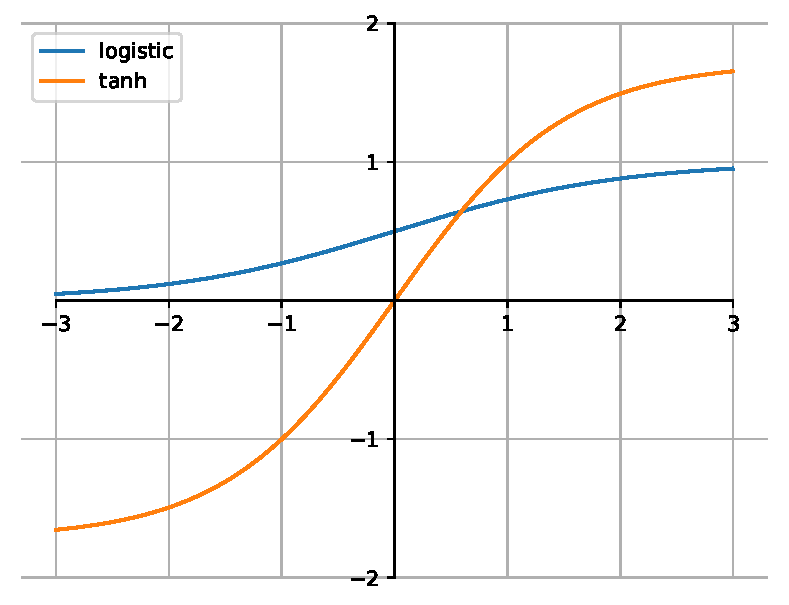
\includegraphics[width=0.8\columnwidth]{plots/logistic_vs_tanh_function.pdf}
  \caption{Graph of the logistic sigmoid function and $\tanh$ sigmoid function.}
  \label{fig:logistic_vs_tanh_function}
\end{figure}

A comparison of the performance of both sigmoid functions for our network is shown in \Cref{fig:logistic_vs_tanh}. Note that we adjusted the learning rate for the logistic sigmoid to compensate for the fact that its error function is $(2 \cdot 1.7159)^2$ times smaller than that of the hyperbolic tangent sigmoid.
We can see that using the hyperbolic tangent sigmoid leads to faster convergence compared to using the logistic sigmoid, as expected.

\begin{figure}[!htb]
  \centering
  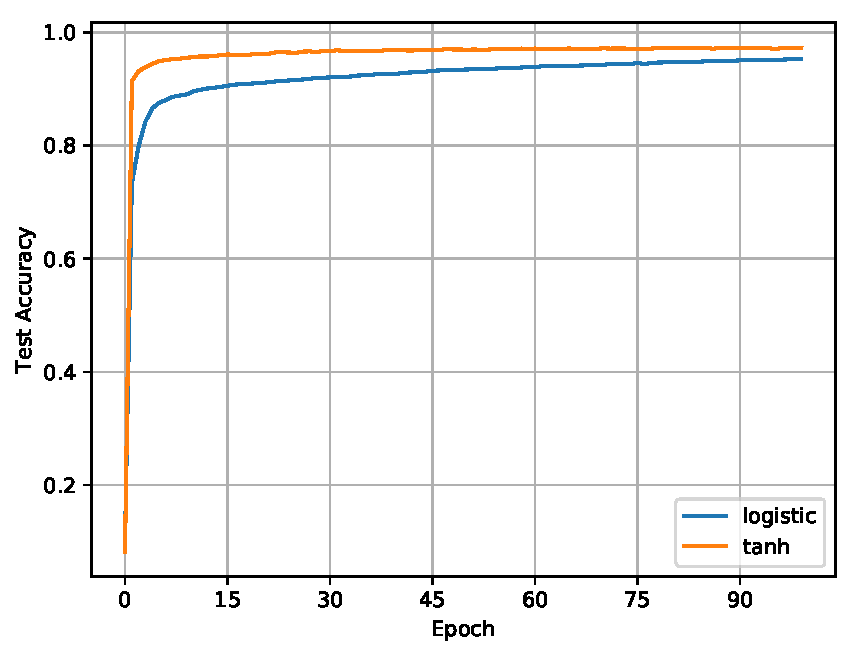
\includegraphics[width=0.8\columnwidth]{plots/logistic_vs_tanh.pdf}
  \caption{Test accuracy when using the logistic sigmoid versus the $\tanh$ sigmoid over $100$ epochs.}
  \label{fig:logistic_vs_tanh}
\end{figure}

\subsection{Weight Initialization}

To ensure that the average input to each layer in the network is close to zero, the weights must also be properly initialized. Given that the input is normalized and that the hyperbolic tangent sigmoid is used, the initial weights should be drawn from a distribution with a standard deviation of $\sigma_w$ as given by \Cref{eq:weight_init}, where $m$ is the fan-in of the layer \cite{lecun_efficient_1998}. We chose to use a Gaussian distribution to select the initial weights.

\begin{equation} \label{eq:weight_init}
\sigma_w = m^{-1/2}
\end{equation}

\subsection{Learning Rate}

The weight update equation for a node $i$ is given by \Cref{eq:weight_update}, where $w_i$ and $\eta_i$ are the weight and learning rate of node $i$, respectively.

\begin{equation} \label{eq:weight_update}
w_i \leftarrow w_i - \eta_i \frac{\partial E}{\partial w_i}
\end{equation}

We initially used a global learning rate $\eta$ for all layers. The learning curve for various values of $\eta$ is shown in \Cref{fig:learning_rate}. This graph shows that a learning rate that is too high, such as $0.1$, causes slow, jagged and non optimal convergence.

\begin{figure}[!htb]
  \centering
  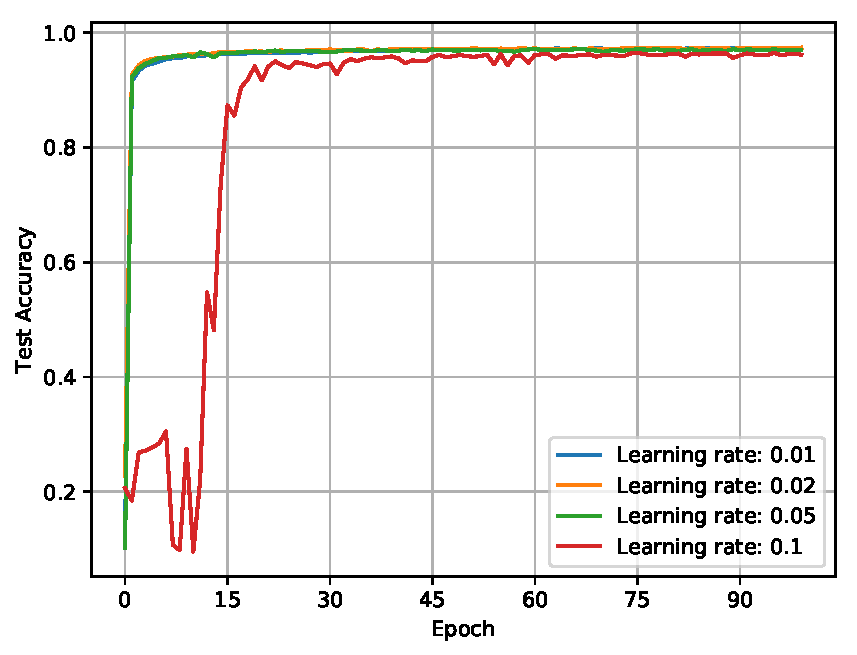
\includegraphics[width=0.8\columnwidth]{plots/learning_rate.pdf}
  \caption{Test accuracy when using various learning rates over $100$ epochs.}
  \label{fig:learning_rate}
\end{figure}

A closer view of the curves for better performing learning rates is shown in \Cref{fig:learning_rate_zoom}. Here, we can see that the learning rate of $0.02$ has the best performance, since it causes quick convergence to a high test accuracy.

\begin{figure}[!htb]
  \centering
  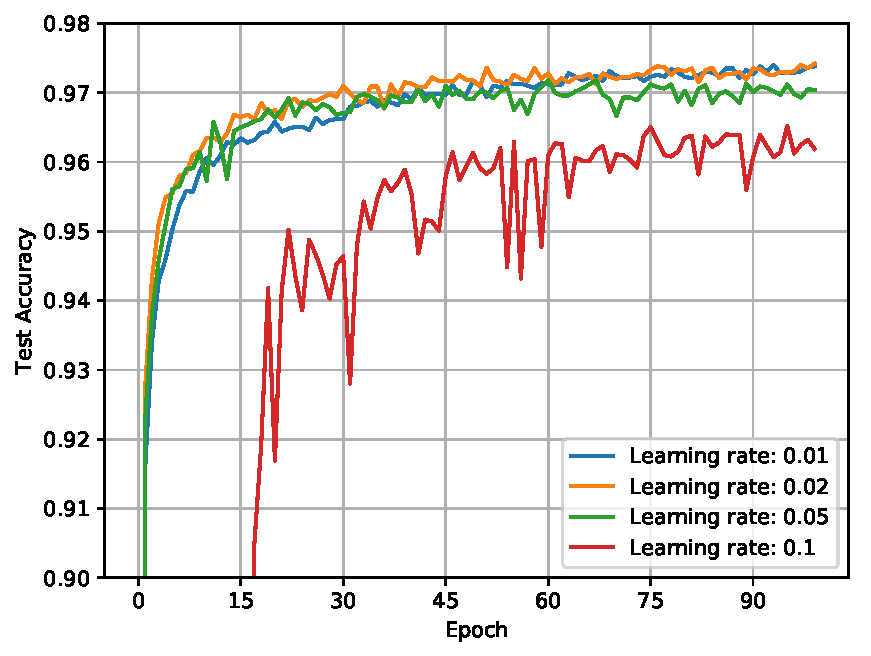
\includegraphics[width=0.8\columnwidth]{plots/learning_rate_zoom_2.pdf}
  \caption{Test accuracy when using various learning rates over $100$ epochs. Cropped to show test accuracies in the $0.90$ to $0.98$ range.}
  \label{fig:learning_rate_zoom}
\end{figure}

\subsection{Layer Decay}

During training, the weight updates will typically be larger in the higher layers of the network. This is due to the fact that the second derivative of the cost function is generally larger in these higher layers \cite{lecun_efficient_1998}. To equalize the weight updates across all layers, the learning rate can be made a decreasing function of the layer depth, with the lower layers having a higher learning rate than the higher ones. This can be implemented with a layer decay term $\delta$, as given by \cref{eq:layer_decay}, where $\eta_i$ is the learning rate in layer $i$, and layer $i$ is higher than layer $i-1$.

\begin{equation} \label{eq:layer_decay}
\eta_i = \delta \eta_{i-1}
\end{equation}

The resulting performance when using various values for the layer decay $\delta$ is shown in \Cref{fig:layer_decay_zoom}. We can see that the layer decay does not have a significant effect on the convergence. This is most likely due to the fact that the network has only one hidden layer. The effect would be more pronounced in much deeper networks.

\begin{figure}[!htb]
  \centering
  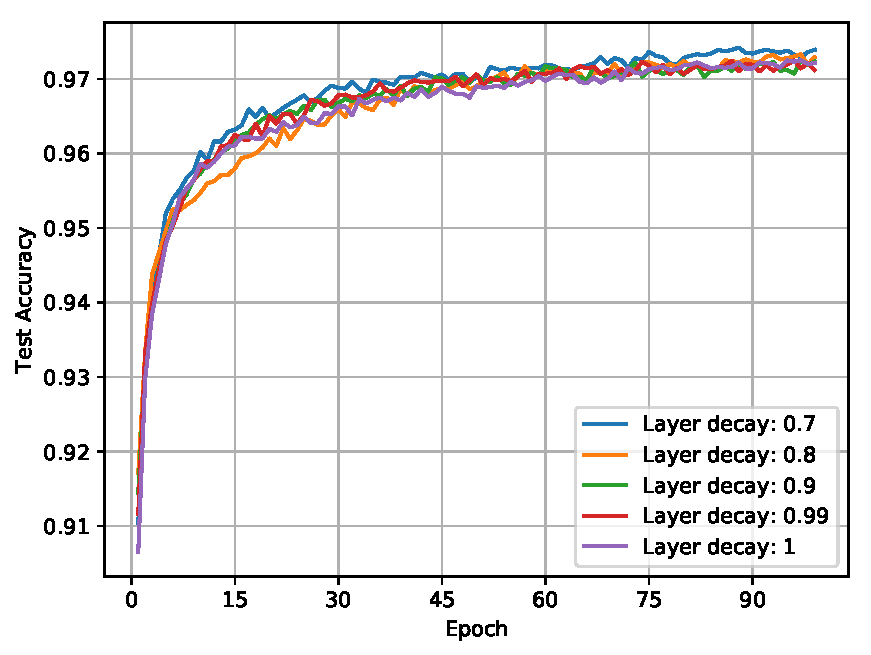
\includegraphics[width=0.8\columnwidth]{plots/layer_decay_zoom.pdf}
  \caption{Test accuracy when using various layer decay values over $100$ epochs.}
  \label{fig:layer_decay_zoom}
\end{figure}

\subsection{Momentum}

Momentum is an added term to the weight update equation that typically helps accelerate convergence \cite{lecun_efficient_1998}. The update equation for the weight change $\Delta w$ is given by \Cref{eq:momentum}, where $\mu$ is the momentum.

\begin{equation} \label{eq:momentum}
\Delta w(t + 1) \leftarrow - \eta \nabla E + \mu \Delta w(t)
\end{equation}

The results of using various values for the momentum $\mu$ are shown in \Cref{fig:momentum}. We can see that, with a high momentum value of $0.9$, the learning curve rises quickly, but does not converge to a global optimum. An intermediate momentum value of $0.3$ leads to relatively fast convergence to a high test accuracy.

\begin{figure}[!htb]
  \centering
  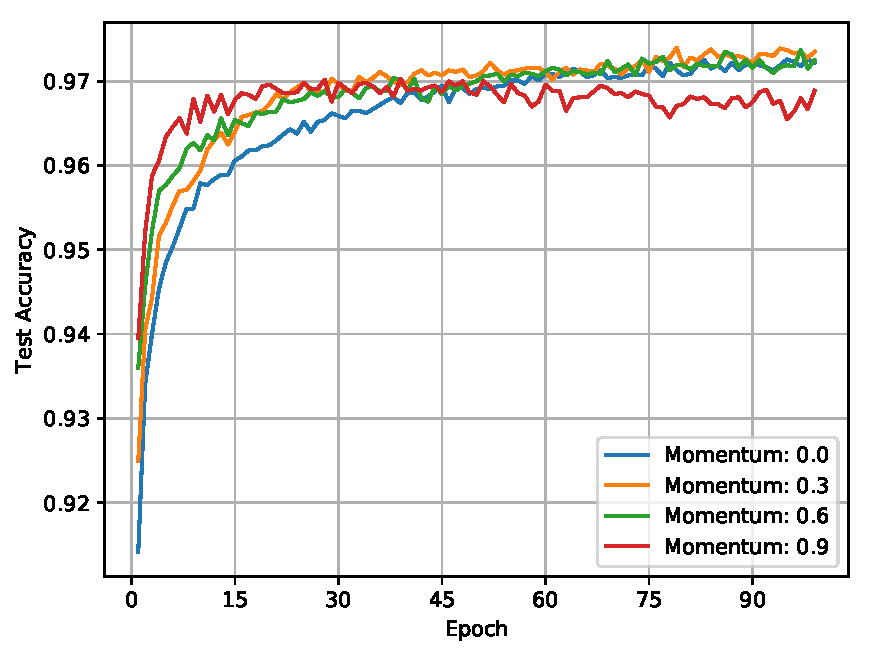
\includegraphics[width=0.8\columnwidth]{plots/momentum_zoom.pdf}
  \caption{Test accuracy when using various momentum values over $100$ epochs.}
  \label{fig:momentum}
\end{figure}

\subsection{Batch Size}

The batch size represents the number of input examples to consider for a single weight update in stochastic gradient descent. This is sometimes referred to as a ``mini-batch'' size. A batch size of $1$ is equivalent to online stochastic gradient descent, where each training example is used for a weight update.

The results of using various batch sizes are shown in \Cref{fig:batch_size}. We can see that a batch size of $1$ leads to very jagged learning. In general, a higher batch size leads to more accurate weight updates, but slower convergence. This can be seen in the discrepancy between the learning curves with batch sizes of $10$ and $100$. Here, the best batch size appears to be $100$, since it causes relatively fast convergence to a high test accuracy.

\begin{figure}[!htb]
  \centering
  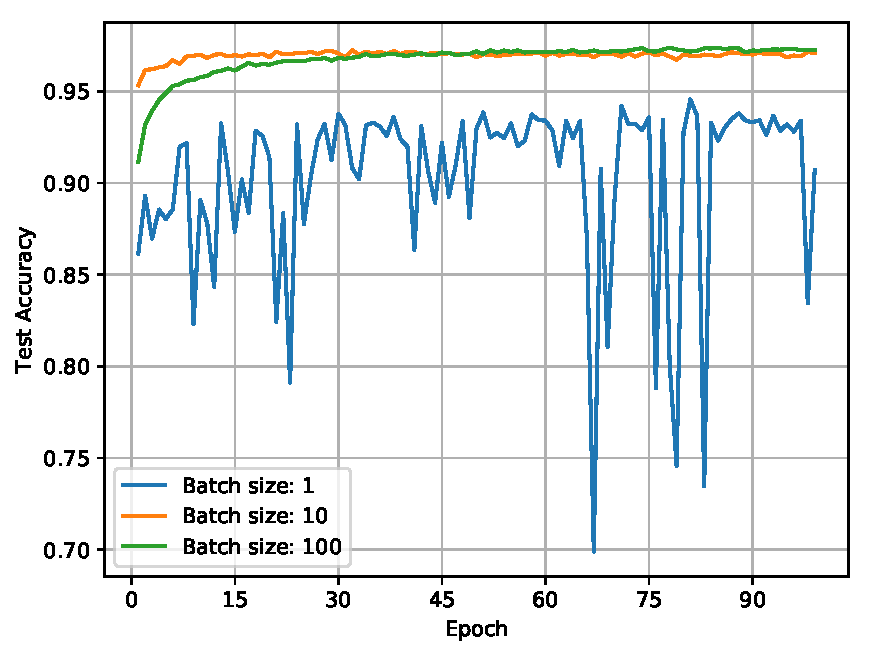
\includegraphics[width=0.8\columnwidth]{plots/batch_size_zoom.pdf}
  \caption{Test accuracy when using various batch sizes over $100$ epochs.}
  \label{fig:batch_size}
\end{figure}

\subsection{Network Size}

With the network tuned to use all the previously described improvements, we tested the effect of varying the network size. The results are shown in \Cref{fig:network_size}. The general trend is that increasing the number of hidden units improves performance. We can see, however, that increasing the number of layers does not yield any significant improvement. The best performing network arrangement is thus one with a single hidden layer with $300$ hidden units.

\begin{figure}[!htb]
  \centering
  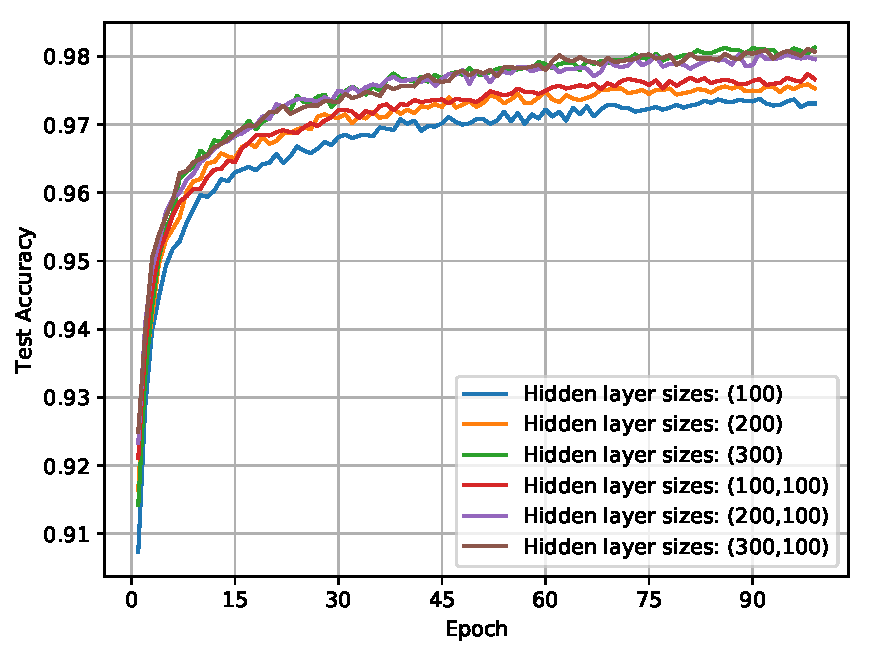
\includegraphics[width=0.8\columnwidth]{plots/network_size_zoom.pdf}
  \caption{Test accuracy when using various hidden layer configurations.}
  \label{fig:network_size}
\end{figure}

\section{Comparison to Other Approaches}

We next compared our best performing network, which contains one hidden layer with $300$ units, to a deep convolutional network taken from TensorFlow \cite{tensorflow} and a random baseline. We expected that a convolutional network would significantly outperform the fully connected network since the features learned by a convolutional layer are applicable to the entire image. Thus, the classifier exhibits some translational invariance to its input and is better suited to image recognition. This is shown clearly in \Cref{fig:network_comparison}, where the convolutional network attains a test accuracy of \SI{99.3}{\percent} compared to the fully connected test accuracy of \SI{98.1}{\percent}. Both of these approaches are still much better than the random baseline, which achieves an expected accuracy of \SI{10}{\percent} and thus was not shown.

\begin{figure}[!htb]
  \centering
  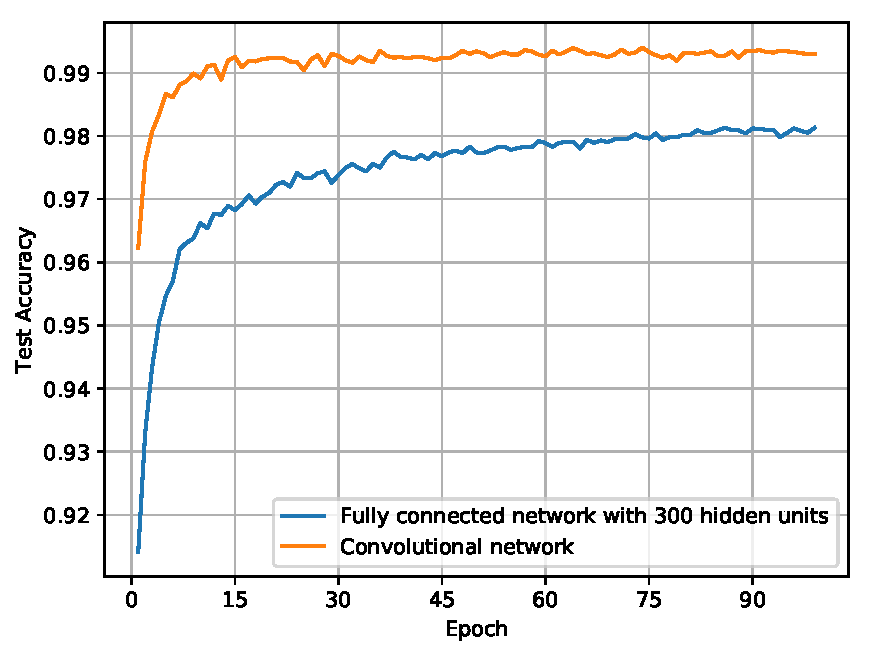
\includegraphics[width=0.8\columnwidth]{plots/network_comparison.pdf}
  \caption{Test accuracy when using a fully connected network with $300$ hidden units and a deep convolutional network.}
  \label{fig:network_comparison}
\end{figure}

\section{Conclusions}

In conclusion, we compared the effects of different tricks on the convergence and performance of the back propagation algorithm applied to a fully connected neural network. Some tricks, such as normalizing the input and using a hyperbolic tangent activation function to reduce biases in learning, and using a larger batch size to better approximate the true gradient, were shown to be effective. Others, such as using a learning rate reduction for higher layers, were found to have little effect for a shallow network. One possible expansion of this study would be to measure the effects of the different tricks for deeper networks. This would likely require the addition of the rectified linear activation function (ReLU), as well as measures to control overfitting such as the addition of dropout layers, in order to obtain reasonable training times and avoid problems like the vanishing gradient experienced by deeper networks.

\bibliographystyle{IEEEtran}
\bibliography{IEEEabrv,references}

\end{document}
